\documentclass{beamer}
\usepackage[T1]{fontenc}
\usepackage[utf8]{inputenc}
\usepackage[francais]{babel}
\usepackage{lmodern}
\usepackage{url}

\title{Contribuons au Libre}
\author{Sébastien Wilmet}
\date{22 février 2012}
\institute{LouviLUG}

\usetheme{Warsaw}

\begin{document}

\begin{frame}
  \titlepage
\end{frame}

\begin{frame}{Sommaire}
  \tableofcontents[hideallsubsections]
\end{frame}

\section{Choses de base}
\begin{frame}
  \tableofcontents[sectionstyle=show/shaded, hideothersubsections]
\end{frame}

\subsection{En parler autour de soi}
\begin{frame}{En parler autour de soi}
  Expliquer :
  \begin{itemize}
    \item les 4 libertés fondamentales ;
    \item ce qu'est GNU/Linux ;
    \item …
  \end{itemize}
\end{frame}

\begin{frame}{Les 4 libertés fondamentales}
  Un Logiciel Libre a 4 libertés fondamentales :
  \begin{itemize}
    \item utilisation sans aucune restriction ;
    \item étudier le fonctionnement du logiciel ;
    \item redistribuer des copies ;
    \item améliorer le programme et redistribuer ces améliorations.
  \end{itemize}
\end{frame}

\subsection{Aider les autres}
\begin{frame}{Aider les autres}
  Aider selon nos connaissances :
  \begin{itemize}
    \item notre entourage ;
    \item organiser une install-party ;
    \item sur un forum ou mailing-list ;
    \item etc.
  \end{itemize}
\end{frame}

\section{Tests de logiciels}
\begin{frame}
  \tableofcontents[sectionstyle=show/shaded, hideothersubsections]
\end{frame}

\subsection{Rapports de bugs}
\begin{frame}{Upstream / Downstream}
  \textit{Upstream} (en amont) = le \textbf{logiciel}\\
  \textit{Downstream} (en aval) = la \textbf{distribution}

  \bigskip
  Bug \textit{downstream} : mauvaise intégration.

  \bigskip
  Hésitation bug \textit{upstream} ou \textit{downstream} ?\\
  $ \Rightarrow $ Rapporter le bug en \textit{downstream}.
\end{frame}

\begin{frame}{Bugtracker}
  Bugtracker : gestion des bugs et demandes de fonctionnalités

  \bigskip
  Exemples \textit{downstream} :
  \begin{itemize}
    \item Fedora : \url{https://bugzilla.redhat.com/}
    \item Ubuntu : \url{https://launchpad.net/ubuntu}
  \end{itemize}

  \bigskip
  Exemple \textit{upstream} :
  \begin{itemize}
    \item GNOME : \url{https://bugzilla.gnome.org/}
  \end{itemize}
\end{frame}

\begin{frame}{Que faire en cas de bug ?}
  \begin{itemize}
    \item Déjà rapporté \textit{downstream} (pour notre distribution) ?
    \item Déjà rapporté \textit{upstream} ?
    \medskip
    \item Si oui, puis-je apporter plus d'informations ?
    \item Si non, décrire précisément les différentes étapes.
  \end{itemize}
\end{frame}

\subsection{Demandes de fonctionnalités}
\begin{frame}{Demandes de fonctionnalités}
  Les développeurs ne connaissent pas les besoins de chacun.

  \bigskip
  Déjà implémenté ? (fichier NEWS, ChangeLog, …)

  \medskip
  Déjà prévu ? (Roadmap, TODO, …)
\end{frame}

\section{Documentation et traduction}
\begin{frame}
  \tableofcontents[sectionstyle=show/shaded, hideothersubsections]
\end{frame}

\subsection{Documentation}
\begin{frame}{Documentation}
  Une bonne documentation est très important.

  \bigskip
  Type de documentation :
  \begin{itemize}
    \item Manuel complet
    \item FAQ : \textit{Frequently Asked Questions}
    \item Par topiques
    \item …
  \end{itemize}
\end{frame}

\subsection{Traduction}
\begin{frame}{Traduction}
  Outil gettext :
  \begin{enumerate}
    \item Marquer dans le code les phrases à traduire ;
    \item Générer un fichier *.pot ;
    \item Un fichier *.po par langue, à compléter ;
  \end{enumerate}

  \bigskip
  Très facile pour le traducteur.
\end{frame}

\begin{frame}{Interfaces web}
  Pour gérer des gros projets comme GNOME :
  \begin{itemize}
    \item statistiques pour chaque langue ;
    \item réserver certaines parties, pour éviter le travail en double ;
    \item etc.
  \end{itemize}
\end{frame}

\section{Création de paquets}
\begin{frame}
  \tableofcontents[sectionstyle=show/shaded, hideothersubsections]
\end{frame}

\begin{frame}{Création de paquets}
  Avantages d'un paquet :
  \begin{itemize}
    \item Ne pas devoir compiler à la main ;
    \item Meilleure intégration à notre distribution ;
    \item Mises à jour et désinstallation plus facile.
  \end{itemize}

  \pause
  \bigskip
  Différents formats :
  \begin{itemize}
    \item \texttt{RPM} : Fedora, Mageia, OpenSuse, …

    \medskip
    \item \texttt{DEB} : Debian, Ubuntu, Mint, …

    \medskip
    \item autres : Gentoo, Arch Linux, …
  \end{itemize}
\end{frame}

\section{Développement}
\begin{frame}
  \tableofcontents[sectionstyle=show/hide, hideothersubsections]
\end{frame}

\subsection{Gestionnaires de versions}
\begin{frame}{Gestionnaires de versions}
  \begin{itemize}
    \item Faciliter la gestion d'un projet de programmation ;
    \item Garder l'historique de toutes les modifications (\textit{commits}) ;
    \item Travailler en équipe ;
    \item Avoir des branches de développement :
      \begin{itemize}
        \item pour développer une fonctionnalité séparément ;
        \item pour une certaine version (2.4.0 $\rightarrow$ 2.4.1 $\rightarrow$ ...).
      \end{itemize}
  \end{itemize}

  \bigskip
  \begin{center}
    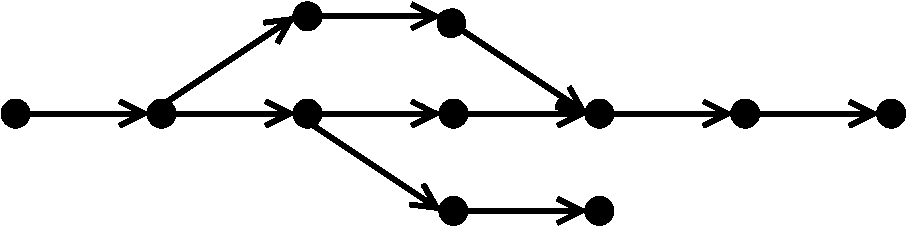
\includegraphics[scale=0.4]{images/commit-branch.pdf}
  \end{center}
\end{frame}

\subsection{Prérequis pour se lancer}
\begin{frame}{Prérequis pour se lancer}
  Maitriser les outils :
  \begin{itemize}
    \item ligne de commandes ;
    \item éditeur de texte (Vim p.~ex.) ;
    \item gestionnaire de versions ;
    \item etc.
  \end{itemize}

  \bigskip
  Bonnes pratiques de programmation (code propre, …) :
  \begin{itemize}
    \item p.~ex. : livre \textit{Code Complete}, McConnell
  \end{itemize}
\end{frame}

\subsection{Se lancer}
\begin{frame}{Se lancer}
  C'est mieux de contribuer à un projet existant.

  \bigskip
  Bien suivre les instructions :
  \begin{itemize}
    \item style du code ;
    \item manière d'envoyer notre contribution (le patch).
  \end{itemize}

  \bigskip
  Opportunité : Google Summer of Code.
\end{frame}

\begin{frame}{Conclusion}
  Il y a plein de moyens de contribuer au Libre, selon nos envies, nos connaissances et notre temps libre.

  \bigskip
  C'est une expérience très enrichissante !

  \bigskip
  \begin{center}
    \textbf{{\Large Des remarques, des questions ?}}
  \end{center}
\end{frame}

\end{document}
